\chapter{Kalman-Filter}
\label{chap:KalmanFilter}

The second approach for a sensor fusion is the Kalman filter. This filter is based on the state space modelling where between the dynamic of the system and the process of the measurement is differentiated. Although the measuring is faulty and the systemstate is noisy, this filter guesses with the help of a set of equations the correct true state of the system. Instead of using the absolut value it uses the meanvalue and variance of the normal distribution. The meanvalue is the perfect measurement and the variance tells the uncertainty of the measurement. Figure \ref{fig:measurement} shows a mesurement of an acceleration sensor.
\begin{figure}[H]
	\centering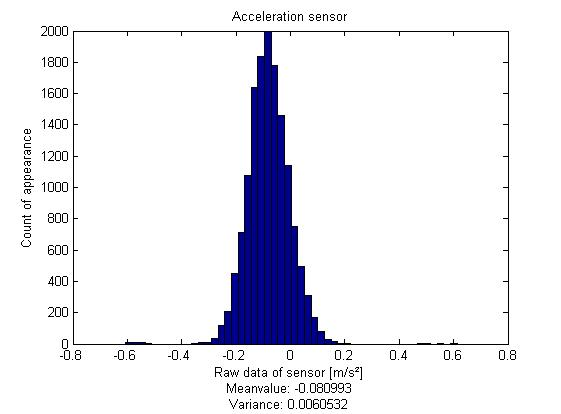
\includegraphics[width=0.8\textwidth]{fig/AccX.jpg}
	\caption{Variance and Meanvalue of an acceleration sensor}
	\label{fig:measurement}
\end{figure}

The following state space description shows the calculation of the new states which in the case of this project represent the angles pitch, roll and yaw. Equation \ref{equ:states} shows the defined state vector.
\begin{align}
\vec x = \begin{pmatrix} pitch \\ roll \\ yaw \end{pmatrix}
\label{equ:states}
\end{align}
The calculation of a new state and the output can be seen in the formulas \ref{equ:KalmanModell1} and \ref{equ:KalmanModell2}.
\begin{align}
\vec{x_k} = \underline{A}\vec x_{k-1}+\underline{B}\vec u_{k-1} + W_{k-1}
\label{equ:KalmanModell1}
\end{align}
\begin{align}
\vec y_k = \underline{H}\vec x_k+ V_k
\label{equ:KalmanModell2}
\end{align}
Legend of the formula shown above:\\
\begin{itemize}
	\item $\vec{x}_k$ state vector of actual step
	\item $\vec{x}_{k-1}$ state vector of previous step
	\item $\underline{A}$ system matrix
	\item $\underline{B}$ input matrix
	\item $\vec{u}_{k-1}$ input vector of previous step
	\item $\underline{W}$ process noise
	\item $\vec{y}_{k}$ output vector
	\item $\underline{H}_k$ output matrix
	\item $\underline{V}$ measurement noise
\end{itemize}
Because of the measurement and the process noise the new state is not good. The Kalman filter takes the process and measurement noise into account to improve the state estimation. To do so the Kalman filter is splitted into two parts, the prediction process (time update) and correction process (measurement update). In the prediction process the filter estimates the states in the next step and calculates the new covariance. Those values are calculated for the states which in the following step are expected to be reached. In the next step the correction update, the filter checks if the precalculated state is reached. According to the difference the correction for the following prediction is done.\\\\
\underline{Prediction step:}\\\\
Predict the next state:
\begin{align}
\vec x_k = \underline{A}\vec x_{k-1}+\underline{B}\vec u_{k-1}
\label{equ:Kalman1}
\end{align}
Predict the covariance for the next step:
\begin{align}
\underline{P}_k = \underline{A}\underline{P}_{k-1}\underline{A}^T+\underline{Q}
\label{equ:Kalman2}
\end{align}



\underline{Correction step:}\\\\
Computation of the Kalman gain:
\begin{align}
\underline{K}_k = \underline{P}_k	\underline{H}^T(\underline{H}\underline{P}_k\underline{H}^T+\underline{R})^{-1}
\label{equ:Kalman3}
\end{align}
Updating state prediction with new measurement:
\begin{align}
\vec x_k = 	\vec x_k+\underline{K}_k(\vec z_k-\underline{H}\vec x_k)
\label{equ:Kalman4}
\end{align}
Updating the error covariance:
\begin{align}
\underline{P}_k = (\underline{I}-\underline{K}_k\underline{H})\underline{P}_k	
\label{equ:Kalman4}
\end{align}
These steps have to be done more than just ones, so when the correction is finished, the update has to be called again and so on.\\
As can be seen the implementation effort is higher than with the Complementary Filter. Because matrices and matrix operations are needed, more calculation steps are needed and the functionality of the Kalman filter is not as intuitive like with the complementary filter. Also the uncertainty of the process itself and the measurement error needs to be known. Nevertheless the results from the Kalman filter are better than those of the complementary filter. This can be seen in the results showing chapter of this project.
